%%%%%%%%%%%%%%%%%%%% book.tex %%%%%%%%%%%%%%%%%%%%%%%%%%%%%
%
% sample root file for the chapters of your "monograph"
%
% Use this file as a template for your own input.
%
%%%%%%%%%%%%%%%% Springer-Verlag %%%%%%%%%%%%%%%%%%%%%%%%%%


% RECOMMENDED %%%%%%%%%%%%%%%%%%%%%%%%%%%%%%%%%%%%%%%%%%%%%%%%%%%
\documentclass[pdftex,12pt, oneside]{article}

% choose options for [] as required from the list
% in the Reference Guide, Sect. 2.2
\usepackage[paperwidth=8.5in, paperheight=13in]{geometry}

\usepackage{makeidx}         % allows index generation
\usepackage{graphicx}        % standard LaTeX graphics tool
                             % when including figure files
%\usepackage{multicol}        % used for the two-column index
\usepackage[bottom]{footmisc}% places footnotes at page bottom
\usepackage[english]{babel}
\usepackage{enumerate}
\usepackage{paralist}
\usepackage{float}
\usepackage{gensymb}  
\usepackage{listings}
%\usepackage{siunitx}
% etc.
% see the list of further useful packages
% in the Reference Guide, Sects. 2.3, 3.1-3.3
\renewcommand{\baselinestretch}{1.5}

\newcommand{\HRule}{\rule{\linewidth}{0.5mm}}

%\makeindex             % used for the subject index
                       % please use the style svind.ist with
                       % your makeindex program


%%%%%%%%%%%%%%%%%%%%%%%%%%%%%%%%%%%%%%%%%%%%%%%%%%%%%%%%%%%%%%%%%%%%%

\begin{document}

%\author{Priyanto Tamami}
%\title{BUKU PETUNJUK OPERASIONAL SISTEM INFORMASI GEOGRAFIS UNTUK PBB-P2 DENGAN MAPINFO VERSI 8.0}
%\date{22 Desember 2015}
%\maketitle

%\input{./01.title.tex}
\begin{center}
{\large PROPOSAL STUDI KELAYAKAN PENGOLAHAN DATA SISTEM INFORMASI PAJAK BUMI DAN BANGUNAN PERDESAAN DAN PERKOTAAN BERBASIS WEB}
\\[1cm]
10 Februari 2016\\
Priyanto Tamami, S.Kom.
\end{center}

%\frontmatter%%%%%%%%%%%%%%%%%%%%%%%%%%%%%%%%%%%%%%%%%%%%%%%%%%%%%%

%\include{dedic}
%\include{pref}

%\include{02.pengesahan} 

%\tableofcontents
%\listoffigures

%\mainmatter%%%%%%%%%%%%%%%%%%%%%%%%%%%%%%%%%%%%%%%%%%%%%%%%%%%%%%%
%\include{part}
%\include{chapter}
%\include{chapter}
%\appendix
%\include{appendix}

%\include{03.konsep-sig}
%\include{04.pengenalan-software}
%\include{05.koordinat}
%\include{06.registrasi-transformasi-koordinat} 
%\include{07.digitasi-on-screen} 
%\include{08.query} 

%\backmatter%%%%%%%%%%%%%%%%%%%%%%%%%%%%%%%%%%%%%%%%%%%%%%%%%%%%%%%
%\include{solutions}
%\include{referenc}
%\printindex

%%%%%%%%%%%%%%%%%%%%%%%%%%%%%%%%%%%%%%%%%%%%%%%%%%%%%%%%%%%%%%%%%%%%%%

\section{LATAR BELAKANG MASALAH}

Pada saat ini teknologi komputer berkembang dengan pesat seiring dengan laju pertumbuhan jaman, termasuk di dalamnya adalah perkembangan teknologi jaringan informasi. Dengan masuknya manusia kepada peradaban teknologi informasi, dimana manusia sangat bergantung kepada seberapa cepatnya informasi yang dapat dia peroleh untuk memenuhi kebutuhannya, maka aplikasi berbasis web merupakan salah satu solusi untuk mengatasi keadaan tersebut.

Dengan adanya teknologi aplikasi berbasis web, maka informasi dapat disampaikan dengan cepat walaupun terpisahkan oleh jarak. \textit{Website} yang dulu bersifat statis, dengan kemunculan beragam bahasa pemrograman seperti PHP, Java, ASP, dan aplikasi web lainnya, maka tampilan \textit{website} sekarang jauh lebih dinamis. Ditambah dengan perkembangan teknologi Ajax yang memungkinkan halaman sebuah \textit{website} lebih ringan untuk diakses serta dapat memberikan informasi secara \textit{realtime} dengan penggunaan \textit{bandwidth} internet yang cukup efektif dan efisien.

Dalam perkembangan pelayanan publik yang dilaksanakan oleh Pemerintahan Daerah, tidak terlepas dari perkembangan teknologi informasi sebagai salah satu sarana yang menghubungkan komunikasi antara Pemerintah Daerah dan masyarakatnya, salah satu sarananya adalah dengan menyediakan suatu halaman \textit{website} yang dapat diakses oleh masyarakat, dimana didalamnya dapat berupa informasi kegiatan-kegiatan apa saja yang telah dilakukan Pemerintah Daerah dalam melaksanakan pembangunan di wilayah Kabupaten Brebes, apa saja agenda yang akan dilaksanakan kedepan, dan berbagai macam informasi yang dapat ditampilkan sebagai salah satu media komunikasi antara Pemerintah Daerah dengan masyarakat.

Pokok masalah dari pengajuan proposal rencana studi ini adalah apakah pembuatan sebuah aplikasi berbasis web yang hadir ditengah masyarakat Kabupaten Brebes ini layak untuk dibangun, ataukah ada solusi-solusi lain bukan hanya dalam rangka Pemerintah Daerah dalam hal ini Dinas Pendapatan dan Pengelolaan Keuangan melakukan komunikasi dengan masyarakat Kabupaten Brebes, tetapi sekaligus dapat melakukan pengawasan penerimaan dari Pajak Bumi dan Bangunan Perdesaan dan Perkotaan yang berlaku di masyarakat.

\section{MAKSUD DAN TUJUAN}

Maksud dan tujuan yang akan dicapai dalam kegiatan studi kelayakan ini cukup sederhana, yaitu menganalisa apakah aplikasi yang akan dikembangkan nantinya layak untuk dipublikasikan dan dibuka untuk diakses oleh masyarakat, karena berkaitan dengan kondisi kerahasiaan data wajib pajak sesuai Undang Undang Nomor 6 Tahun 1983 tentang Ketentuan Umum dan Tata Cara Perpajakan, sebagaimana diubah terakhir dengan Undang Undang Nomor 16 Tahun 2009.

\section{BATASAN MASALAH}

Karena luasnya ruang lingkup dalam pembahasan studi kelayakan ini, maka penyusunan studi kelayakan akan diberikan batasan masalah sebagai berikut :

\begin{enumerate}[1.]
  \item Studi kelayakan ini melihat dari kacamata hukum apakah dengan dibangunnya aplikasi ini tidak bertentangan dengan peraturan yang sudah ada atau tidak.
  
  \item Studi kelayakan ini melihat dari kebutuhan organisasi dalam hal ini instansi pemerintah terhadap suatu aplikasi berbasis web sebagai sarana berkomunikasi dengan masyarakat wajib pajak untuk jenis Pajak Bumi dan Bangunan Perdesaan dan Perkotaan sekaligus menjadi kontrol pembayaran pajak yang dititipkan wajib pajak atau kuasanya kepada pemerintah Desa untuk dibayarkan ke tempat pembayaran yang ditunjuk.
  
\end{enumerate}

\section{PERENCANAAN TARGET}

Target yang akan dicapai dari studi kelayakan ini melihat bahwa apakah kebutuhan pembuatan aplikasi web yang akan menampilkan informasi mengenai status pembayaran Surat Pemberitahuan Pajak Terhutang untuk jenis Pajak Bumi dan Bangunan Perdesaan dan Perkotaan, selain sebagai bentuk keterbukaan informasi kepada wajib pajak sekaligus sebagai kontrol terhadap petugas pemungut tingkat Desa/Kelurahan dalam menyalurkan realisasi penerimaan Pajak Bumi dan Bangunan Perdesaan dan Perkotaan dari wajib pajak atau kuasanya ke Bank Tempat Pembayaran, terhadap pemberlakuan kerahasiaan data wajib pajak pada Undang Undang Nomor 6 Tahun 1983 tentang Ketentuan Umum dan Tata Cara Perpajakan sebagaimana diubah terakhir dengan Undang Undang Nomor 16 Tahun 2009.

\section{PERSIAPAN PENGUMPULAN FAKTA}

Dalam pengumpulan fakta pendukung studi kelayakan ini, karena dasarnya adalah kebutuhan organisasi terhadap beberapa ide dan melihat dari sisi hukum perpajakan yang berlaku, maka bentuknya adalah berupa survey internal mengenai setuju atau tidaknya membangun sebuah aplikasi sistem informasi status pembayaran Pajak Bumi dan Bangunan Perdesaan dan Perkotaan, serta dasar dasar hukum yang menyebutkan hal tentang kerahasiaan data wajib pajak.

\section{PENENTUAN JADWAL WAKTU}

Penentuan jadwal waktu adalah sebagaimana tertera pada grafik gantt berikut ini :

\begin{figure}[H]
  \centering
  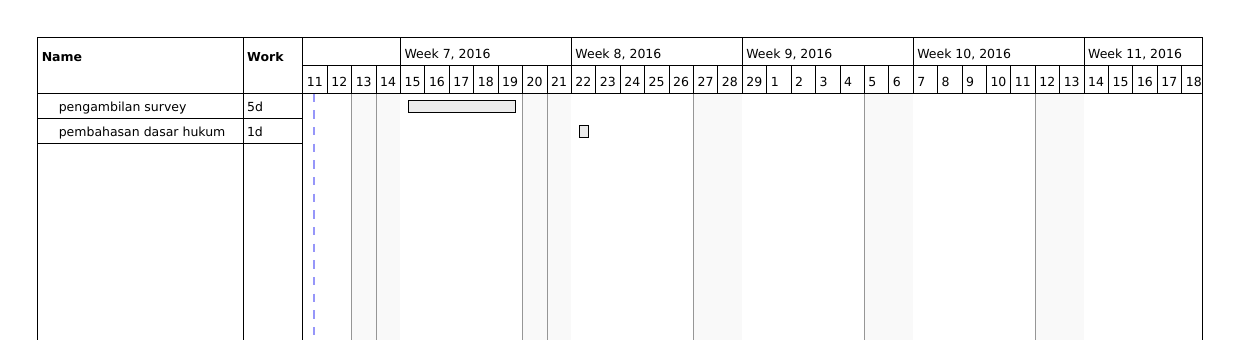
\includegraphics[width=0.7\textwidth]{./resources/jadwal-studi-kelayakan}
  \caption{Jadwal Waktu Studi Kelayakan}
\end{figure}

\section{CAKUPAN KEGIATAN}

Cakupan kegiatan pada studi kelayakan ini hanya memerlukan pengumpulan hasil survey apakah aplikasi yang dibangun ini dianggap perlu atau tidak, serta melihat terhadap produk hukum, apakah aplikasi ini bertentangan atau tidak.

\section{TENAGA DAN BIAYA YANG DIPERLUKAN UNTUK STUDI KELAYAKAN}

Tenaga yang diperlukan untuk studi kelayakan ini hanya 1 (satu) orang fungsional Pranata Komputer sebagai pengolah data hasil survey dan mempelajari aturan aturan mengenai ketentuan umum dan tata cara perpajakan, serta beberapa responden internal yang memberikan keterangan dalam lembar survey.

\end{document}